% Exemple de fichier fonctionnnant avec la classe CAp2012.cls
% Base :
%	Classe pf2010.cls adpatée de pf2003 par Jean CHarlet
%	Classe pf2003.cls adpatée de ic2001 par Jean CHarlet
%
% 	Classe ic2001.cls adpatée de EEGDRI3 par Jean CHarlet
%
% 	Classe EEGDRI3.cls adpatée de ic2000 par Jean CHarlet
%
% 	Classe IC'2000 (ic2000.cls) par Jean Charlet
%
% 	adaptée de la classe IC'99 (afia99.cls) développée par Fabien Torre

%\documentclass{CAp2012}
\documentclass[publibook-draft]{CAp2012}

\newcommand{\verbfichex}{CAp2012.\xspace}
\newcommand{\verbfichclass}{CAp2012.cls\xspace}
\newcommand{\verbfichbst}{CAp2012.bst\xspace}


%\usepackage[pdftex]{pstricks}

\usepackage{verbatim}
\usepackage{subfigure}
\usepackage[french]{babel}
\usepackage[utf8]{inputenc}
\usepackage[T1]{fontenc}
\usepackage{amsmath}
\usepackage{amssymb}
\usepackage{natbib}
%%% francisation des algorithmes


%\newtheorem{algorithm}{Algorithme}
\newtheorem{definition}{Définition}
\newtheorem{lemme}{Lemme}
\newtheorem{theorem}{Théorème}
\newtheorem{hypo}{Hypothèse}
\newtheorem{cor}{Corollaire}
\newtheorem{prop}{Proposition}
\newtheorem{exemple}{Exemple}
\newtheorem{remarques}{Remarques}
\newtheorem{remarque}{Remarque}
\newtheorem{problem}{Problème}
\newtheorem{algo}{Algorithme}
\newtheorem{preuve}{Démonstration}
\newcommand{\argmax}{\operatorname*{argmax}} %\operatorname* pour les op. pouvant admettre des limites...
\newcommand{\argmin}{\operatorname*{argmin}}
\newcommand{\minp}{\operatorname*{min_+}}
\newcommand{\dom}{\operatorname*{dom}}
\newcommand{\Ker}{\operatorname*{Ker}}
\newcommand{\trace}{\operatorname*{trace}}
\newcommand{\cov}{\operatorname{cov}}
\newcommand{\epi}{\operatorname{epi}}
\newcommand{\card}{\operatorname*{Card}}
\newcommand{\conv}{\operatorname*{Conv}}
\newcommand{\vect}{\operatorname*{Vect}}
\newcommand{\var}{\operatorname{Var}}
\newcommand{\diag}{\operatorname{diag}}
\newcommand{\erf}{\operatorname{erf}}
\newcommand{\bound}{\operatorname*{bound}}
\newcommand{\vpi}{\operatorname{VPI}}
\newcommand{\gn}{\operatorname{Gain}}
\newcommand{\p}{\operatorname{Pr}}
\newcommand{\mlp}{\operatorname{MLP}}
\newcommand*\tto[2]{\smash{\mathop{\longrightarrow}\limits_{#1}^{#2}}}
\newcommand*\ntto[2]{\smash{\mathop{\nrightarrow}\limits_{#1}^{#2}}}
\newcommand{\X}{\mathbf{X}}
\newcommand{\Q}{\mathbf{Q}}
\newcommand{\A}{\mathbf{A}}
\newcommand{\Z}{\mathbf{Z}}
\newcommand{\Y}{\mathbf{Y}}
\newcommand{\E}{\mathbf{E}}
\newcommand{\K}{\mathbf{K}}
\newcommand{\F}{\mathcal{F}}
\newcommand{\R}{\mathbf{R}}
\newcommand{\ba}{\mathbf{a}}
\newcommand{\bb}{\mathbf{b}}
\newcommand{\bc}{\mathbf{c}}
\newcommand{\bd}{\mathbf{d}}
\newcommand{\be}{\mathbf{e}}
\newcommand{\af}{\mathbf{f}}
\newcommand{\bg}{\mathbf{g}}
\newcommand{\bh}{\mathbf{h}}
\newcommand{\bi}{\mathbf{i}}
\newcommand{\bj}{\mathbf{j}}
\newcommand{\bk}{\mathbf{k}}
\newcommand{\bl}{\mathbf{l}}
\newcommand{\bm}{\mathbf{m}}
\newcommand{\bn}{\mathbf{n}}
\newcommand{\bo}{\mathbf{o}}
\newcommand{\bp}{\mathbf{p}}
\newcommand{\bq}{\mathbf{q}}
\newcommand{\br}{\mathbf{r}}
\newcommand{\bs}{\mathbf{s}}
\newcommand{\bt}{\mathbf{t}}
\newcommand{\bu}{\mathbf{u}}
\newcommand{\bv}{\mathbf{v}}
\newcommand{\bw}{\mathbf{w}}
\newcommand{\bx}{\mathbf{x}}
\newcommand{\by}{\mathbf{y}}
\newcommand{\bz}{\mathbf{z}}
\newcommand{\ma}{\mathbf{A}}
\newcommand{\mb}{\mathbf{B}}
\newcommand{\mc}{\mathbf{C}}
\newcommand{\md}{\mathbf{D}}
\newcommand{\me}{\mathbf{E}}
\newcommand{\mf}{\mathbf{F}}
\newcommand{\mg}{\mathbf{G}}
\newcommand{\mh}{\mathbf{H}}
\newcommand{\mi}{\mathbf{I}}
\newcommand{\mj}{\mathbf{J}}
\newcommand{\mk}{\mathbf{K}}
\newcommand{\ml}{\mathbf{L}}
\newcommand{\mm}{\mathbf{M}}
\newcommand{\mn}{\mathbf{N}}
\newcommand{\mo}{\mathbf{O}}
\newcommand{\Mp}{\mathbf{P}}
\newcommand{\mq}{\mathbf{Q}}
\newcommand{\mr}{\mathbf{R}}
\newcommand{\ms}{\mathbf{S}}
\newcommand{\mt}{\mathbf{T}}
\newcommand{\Mu}{\mathbf{U}}
\newcommand{\mv}{\mathbf{V}}
\newcommand{\mw}{\mathbf{W}}
\newcommand{\mx}{\mathbf{X}}
\newcommand{\my}{\mathbf{Y}}
\newcommand{\mz}{\mathbf{Z}}
\newcommand{\tphi}{\tilde{\Phi}}
\newcommand{\espace}{\text{ }}
\newcommand{\x}{\mathbf{x}}
\newcommand{\s}{\mathbf{s}}
\newcommand{\n}{\mathbf{n}}
\newcommand{\y}{\mathbf{y}}
\newcommand{\I}{\mathbf{I}}
\newcommand{\rr}{\mathbf{r}}

%%%%%%%%%%%%%%%%%%%%%%%%%%%%%%%%%%%%%%%%%%%%%%%%%%%%%%%%%%%%%%%%%%%%%%%
% Titre court si le titre fait plus de 40 caractères
%%%%%%%%%%%%%%%%%%%%%%%%%%%%%%%%%%%%%%%%%%%%%%%%%%%%%%%%%%%%%%%%%%%%%%%

\shorttitle{Batch Inverse Reinforcement Learning}

\shortouvrage{CAp 2012}

% Titre, auteur, pas de date

\title{Classification structurée pour l'apprentissage par renforcement inverse}

\author{\fontsize{12}{12}\selectfont{Edouard Klein\inst{1}\inst{2}, Matthieu Geist\inst{1}, Olivier Pietquin\inst{1}\inst{3}}}

\institute{
Sup\'elec,\\
IMS Research group, France\\
\texttt{prenom.nom@supelec.fr}
\and
Equipe ABC,\\
LORIA-CNRS, France
\and
UMI 2958\\
GeorgiaTech-CNRS, France
}


\begin{document}
\maketitle


\begin{abstract}
  Cette contribution traite du problème de l'apprentissage par imitation par le biais de l'apprentissage par renforcement inverse ({\it Inverse Reinforcement Learning, IRL}). Dans ce contexte, un expert accomplit une tâche qu'un agent doit essayer de reproduire. L'IRL part du postulat que l'expert optimise avec succès une fonction d'utilité ; le problème consiste à deviner cette fonction (appelée récompense) avec pour entrée une trace du comportement de l'expert. Les algorithmes d'IRL existants nécessitent une ou plusieurs des conditions suivantes pour fonctionner : trajectoires complètes de la part de l'expert, un modèle génératif pour les estimations de type Monte-Carlo, la connaissance des probabilités de transition, la capacité de résoudre le problème direct (celui du {\it Reinforcement Learning, RL}) de manière répétée ou l'accès à la strategie complète de l'expert. Notre contribution consiste en un nouvel algorithme d'IRL levant toutes ces contraintes. En utilisant une méthode supervisée dans laquelle nous introduisons implicitement la structure du processus décisionnel de Markov ({\it Markov Decision Process, MDP}) sous-jacent, nous créons un algorithme basé sur une descente de sous gradient, possèdant une faible complexité tant en échantillons que calculatoire et ne nécessitant pas la résolution du problème direct.
  \motscles{Apprentissage par renforcement, Apprentissage par renforcement inverse, Processus Decisionnel de Markov}
\end{abstract}
%%%%%
\section{Introduction}
%%%%%
\begin{itemize}
\item Introduction informelle sur les processus de décision séquentielles
\item Intérêt de l'apprentissage par démonstration
\item Intérêt de l'IRL pour faire de l'apprenticeship learning
\item Rapide point sur les limitations des algos d'IRL actuels
\begin{itemize}
\item \cite{ng2000algorithms} : Probabilités de transitions devant être connues
\item \cite{abbeel2004apprenticeship} et toutes les approches résumées dans \cite{neu2009training}: Résolution du problème direct à chaque itération
\end{itemize}
\end{itemize}
%%%%%
\section{Background}
%%%%%
\label{back.sec}
%%%
\subsection{Principe}
%%%
Le cadre dans lequel nous plaçons notre étude est celui de la prise de décisions séquentielle. La configuration du système à contrôler est alors décrite à chaque instant $t$ par un état $s_t \in S$. Confronté à cet état, l'agent doit prendre un décision $a_t\in A$. Le système évolue alors vers l'état suivant $s_{t+1}$ selon une certaine probabilité $p(s_{t+1}|s_t, a_t)$. Une politique de contrôle déterministe \footnote{On peut se restreindre au cas déterministe sans perte de généralité} $\pi : S\rightarrow A$ définit le comportement d'un agent confronté à un tel problème de décision séquentielle.\\

Dans le cadre plus restreint de l'apprentissage par renforcement, pour guider la résolution de ce problème il faut fournir à l'agent une fonction de récompense $R : S \rightarrow \mathbb{R}$ qui lui apprendra le degré auquel l'état dans lequel il se trouve est désirable. Une des forces de l'apprentissage par renforcement réside dans le fait que l'agent ne va pas apprendre à maximiser la récompense immédiate mais au contraire un critère prenant le futur en compte. On définit pour ce faire la fonction de valeur $V^\pi$ :
\begin{eqnarray}
\label{Vdef.eqn}
V^\pi(s) &=& E\left[\left.\sum_t\gamma^tR(s_t)\right|s_0=s,\pi\right]\\
&=& R(s) + \gamma\sum_{s'}p(s'|s,\pi(s))V^\pi(s')
\label{BellmanV.eqn}
\end{eqnarray}
où $\gamma$ est un facteur d'actualisation strictement plus petit que $1$. Une politique optimale est alors définie comme une politique dont la fonction de valeur $V^*$ (appelée fonction de valeur optimale) vérifie :
\begin{equation}
\forall \pi, \forall s, V^*(s) \geq V^\pi(s).
\end{equation}
L'ensemble formé par l'espace d'état $S$, l'espace d'action $A$, les probabilités de transition $p$, le facteur $\gamma$ et la fonction de récompense $R$ forme un processus décisionnel de Markov ({\it Markov Decision Process, MDP}).\\

Parfois, définir la fonction de récompense est une tâche ardue alors qu'il est possible à l'opérateur de convenablement contrôler le système de manière intuitive. Un exemple de ce type de tâche est la conduite d'une voiture. Nous accompplissons ce genre de choses au quotidien sans trop y penser mais nous serions bien en peine de préciser les poids précis que nous attribuons aux différents critères tels que la distance nous séparant de la voiture devant nous, la brutalité avec laquelle nous appuyons sur la pédale de frein lorsqu'un danger se présente et ainsi de suite. Dans de tels cas, il est utile d'inférer la récompense à partir d'un comportement démontré.\\

C'est la définition de l'apprentissage par renforcement inverse. Le problème est de retrouver la fonction de récompense optimisée par un expert. Usuellement l'expert est considéré comme un agent optimal dans un MDP et l'on a accès ou bien à la politique complète $\pi_E$ de l'expert ou bien à quelques trajectoires tirées selon cette politique.\\

Ce problème est mal posé dans la mesure où étant donné un comportement, il n'y a pas unicité de la récompense pour lequel ce comportement est optimal. Particulièrement, la récompense uniformément nulle remplit ce critère dans la mesure où tout comportement est optimal vis à vis de cette récompense.
%%%
\subsection{Considérations techniques}
\label{ConsiderationsTechniques.sec}
%%%
La recherche de la politique optimale en apprentissage par renforcement se fait souvent en utilisant une fonction voisine de la fonction de valeur, la fonction de qualité définie par :
\begin{eqnarray}
Q^\pi(s,a) &=& E\left[\left.\sum_t\gamma^tR(s_t)\right|s_0=s,a_0=a,\pi\right]\\
&=& R(s) + \gamma\sum_{s'}p(s'|s,a)V^\pi(s').
\end{eqnarray}
La politique optimale se définit simplement à partir de la fonction de qualité optimale $Q^*$ via un mécanisme glouton :
\begin{equation}
\label{greedy.eqn}
\pi^*(s) \in \arg\max_a Q^*(s,a).
\end{equation}
Dès lors, l'approximation de la fonction de valeur (terme qui employé au sens large désigne aussi la fonction de qualité) est un thème central en apprentissage par renforcement. Une caractéristique répandue dans la litérature est l'utilisation d'un cadre d'approximation linéaire où, après avoir défini des attributs vectoriels $\phi: S\times A \rightarrow \mathbb{R}^k$, l'on va chercher un vecteur de paramètres $\omega$ tel que l'on ait une bonne approximation de la fonction de qualité :
\begin{equation}
\hat Q (s,a) = \omega^T\phi(s,a)\approx Q(s,a).
\end{equation}
Il est naturel d'adopter le même type d'approche pour l'apprentissage par renforcement inverse, c'est à dire de considérer que l'inconnue du problème, la récompense $R$, peut être bien approximée grâce à un vecteur de poids $\theta$ et des attributs vectoriels $\psi : S\rightarrow \mathbb{R}^p$ :
\begin{equation}
\label{hatRdef.eqn}
\hat R(s) = \theta^T\psi(s)\approx R(s).
\end{equation}

Introduire cette expression dans la définition de la fonction de valeur (Equation \ref{Vdef.eqn}) fait apparaître un terme intéressant et dont l'usage est assez répandu dans les algorithmes existants :
\begin{eqnarray}
V^\pi(s) &=& E\left[\left.\sum_t\gamma^t\theta^T\psi(s_t)\right|s_0=s,\pi\right]\\
V^\pi(s) &=& \theta^TE\left[\left.\sum_t\gamma^t\psi(s_t)\right|s_0=s,\pi\right]\\
V^\pi(s) &=& \theta^T\mu^\pi(s)
\label{Vmu.eqn}
\end{eqnarray}

Le terme $\mu^\pi$ est appelé la {\it feature expectation} d'une politique. Il existe plusieurs variantes basées sur la même définition que nous venons de donner. Dans sa version la plus spécifique, notée simplement $\mu^\pi$, il s'agit en toute rigueur de l'expression :
\begin{eqnarray}
\label{mupidef.eqn}
\mu^\pi = E\left[\left.\sum_t\gamma^t\psi(s_t)\right|s_0\sim d,\pi\right],
\end{eqnarray}
où $d$ est une distribution sur l'état initial. Il peut également être utile de le définir sous la forme $\mu^\pi(s,a)$ où son rôle par rapport à $\mu^\pi(s)$ est le même que celui de $Q$ par rapport à $V$ :
\begin{eqnarray}
\mu^\pi(s,a) = E\left[\left.\sum_t\gamma^t\psi(s_t)\right|s_0=s,a_0=a,\pi\right].
\end{eqnarray}
C'est d'ailleurs cette variante de l'expression qui sera utilisée si, au lieu d'injecter l'équation \ref{hatRdef.eqn} dans la définition de la fonction de valeur comme nous l'avons fait pour obtenir l'équation \ref{Vmu.eqn}, nous l'injectons dans la définition de la fonction de qualité. On obtient alors :
\begin{eqnarray}
Q^\pi(s,a) &=& E\left[\left.\sum_t\gamma^t\theta^T\psi(s_t)\right|s_0=s,a_0=a,\pi\right]\\
 &=& \theta^TE\left[\left.\sum_t\gamma^t\psi(s_t)\right|s_0=s,a_0=a,\pi\right]\\
 &=& \theta^T\mu^\pi(s,a)
\label{Qmu.eqn}
\end{eqnarray}

On peut noter que si deux politiques ont la même {\it feature expectation}, alors ces deux politiques ont la même valeur vis à vis de la récompense, quel que soit le vecteur de poids $\theta$ définissant celle-ci. En effet
\begin{eqnarray}
\mu^{\pi_1} = \mu^{\pi_2} &\Rightarrow& \theta^T\mu^{\pi_1} = \theta^T\mu^{\pi_2}\\
& \Rightarrow& V^{\pi_1} = V^{\pi_2}.
\label{memevaleur.eqn}
\end{eqnarray}
La {\it feature expectation} de l'expert, $\mu_E$, pouvant être calculée sans forcément avoir accès à l'intégralité de la politique $\pi_E$, certains algorithmes de la litérature ont, comme nous allons le voir, pour objectif de minimiser la distance entre les {\it feature expectations} respectives de l'agent et de l'expert, afin d'obtenir un agent dont le comportement à la même valeur que celui de l'expert.
%%%%%
\section{Loss-augmented Feature Expectation Matching}
%%%%%
%%%
\subsection{Principe}
%%%
L'un des postulats de base de l'apprentissage par renforcement inverse est que l'expert est un agent \emph{optimal} vis à vis d'une certaine fonction de récompense que l'on cherche à retrouver. Cela implique, comme nous l'avons vu Equation \ref{greedy.eqn}, qu'il existe un mécanisme glouton reliant la politique de l'expert, $\pi_E$ et la fonction de qualité optimale $Q^E_R$ relative à cette fonction de récompense inconnue :
\begin{equation}
\pi_E(s) \in \arg\max_aQ^E_R(s,a).
\end{equation}
Nous allons utiliser cette propriété pour imaginer une fonction de risque dépendante d'une fonction $q$ qui devra partager avec la fonction inconnue $Q^E_R$ la propriété d'optimalité de l'expert que nous venons d'exprimer.\\
Notons $(s_i,a_i)_i$ les échantillons représentant une ou plusieurs trajectoires de l'expert. Il faut que pour chacun de ces échantillons l'on ait :
\begin{equation}
\label{butLAFEM.eqn}
a_i \in \arg\max_aq(s_i,a).
\end{equation}
Notons
\begin{equation}
a^*_i = \arg\max_aq(s_i,a),
\end{equation}
alors le critère exprimé Equation \ref{butLAFEM.eqn} s'écrit $\forall i, q(s_i,a^*_i) = q(s_i,a_i)$. Notre fonction de risque doit pénaliser les cas où $q(s_i,a^*_i)>q(s_i,a_i)$ car alors la fonction $q$ ne permet pas de justifier (au sens de l'équation \ref{greedy.eqn}) le choix $a_i$ de l'expert.\\
Nous introduisons de surcroit une fonction de perte $l : S \times A \rightarrow \mathbb{R}_+$ dans la définition de $a^*_i$ qui devient maintenant :
\begin{equation}
\label{astar.def}
a^*_i = \arg\max_aq(s_i,a) + l(s_i,a).
\end{equation}
La définition de notre fonction de risque peut alors être assemblée en :
  \begin{eqnarray}
   R_N(q) &=& {1\over N} \sum_{i=1}^N\left(\max_{a}(q(s_i,a) + l(s_i,a)) - q(s_i,a_i) \right)\\
   &=& {1\over N} \sum_{i=1}^N\left(q(s_i,a_i^*) + l(s_i,a_i^*) - q(s_i,a_i) \right)
   \end{eqnarray}

Penchons nous sur le rôle de $l$ : cette fonction permet à l'opérateur d'introduire de la connaissance \emph{a priori} dans le système. En effet, minimiser avec succès la fonction de risque avec un choix de $l$ judicieux permet d'imposer à $q$ une structure telle qu'il existe une marge entre l'action choisie par l'expert et la deuxième meilleure action. Ce type d'argument est assez commun dans la litérature (voir Section \ref{biblio.sec}). Par défaut, définir $l(s_i,a) = 1$ si $a\neq a_i$ et $l(s_i,a_i)=0$ fonctionne bien comme le montrent les expériences (Section \ref{exp.sec}) et les critères fournis en sous-section \ref{proof.sec}.\\


Comme nous l'avons vu Equation \ref{Qmu.eqn}, en faisant l'hypothèse d'une représentation linéaire selon certains attributs $\psi : S\rightarrow \mathbb{R}^p$ de la fonction de récompense il est possible d'exprimer la fonction de qualité d'une politique en fonction de la {\it feature expectation} de cette politique. L'expert ne déroge pas à cette règle et notant $\mu_E$ la {\it feature expectation} de l'expert nous pouvons donc faire l'hypothèse que la fonction $q$ que nous recherchons peut s'exprimer sous la forme $q(s,a) = \theta^T\mu_E(s,a)$. Le calcul de ce terme $\mu_E$, bien que présentant quelques subtilités ne pose pas de problème majeurs même lorsque les seules données auquel l'algorithme a accès consistent en une trace de l'expert (cela est expliqué en sous-section \ref{calculmu.sec}). Nous pouvons donc maintenant exprimer notre risque non plus comme une fonction de $q$ mais comme une fonction du vecteur de paramètres $\theta$, vecteur qui définit la récompense (Equation \ref{hatRdef.eqn}).
   \begin{equation}
   R_N(\theta) = {1\over N} \sum_{i=1}^N\left(\theta ^T \mu_E(s_i,a^*_i) + l(s_i,a^*_i) - \theta ^T \mu_E(s_i,a_i) \right)
   \end{equation}
   Il est possible de minimiser ce risque grâce à la règle d'update qui suit, comme cela est expliqué en section \ref{proof.sec} :
   \begin{equation}
   \theta_{t+1} = \theta_t -\alpha_t{{1\over N}\sum\limits_{i=1}^N\left(\mu_E(s_i,a^*_i) - \mu_E(s_i,a_i)\right)\over ||{1\over N}\sum\limits_{i=1}^N\left(\mu_E(s_i,a^*_i) - \mu_E(s_i,a_i)\right)||_2}.
   \end{equation}
%%%
\subsection{Calcul de $\mu_E$}
%%%
\label{calculmu.sec}
Comme signalé dans la sous-section \ref{ConsiderationsTechniques.sec}, beaucoup d'algorithmes de la littérature reposent sur un calcul de la {\it feature expectation}. Notre algorithme a cependant ceci de particulier qu'il ne nécessite que le calcul de $\mu_E$, la {\it feature expectation} de l'expert et non le calcul de la {\it feature expectation} d'une politique arbitraire. De fait cela nous épargne le besoin d'un simulateur, d'un solveur de MDP ou d'échantillons couvrant tout l'espace d'état.\\

Selon les informations dont on dispose, plusieurs méthodes peuvent être utilisées pour calculer $\mu_E$.\\

Dans le cas le plus facile, on peut utiliser la proximité entre la définition du vecteur $\mu$ (Equation \ref{mupidef.eqn}) et celle de la fonction de valeur (Equation \ref{Vdef.eqn}) pour adapter les algorithmes d'évaluation de la fonction de valeur dans le cadre de la programmation dynamique au calcul de la {\it feature expectation}.\\
En supposant un espace d'état de cardinal fini, l'équation de Bellman (Equation \ref{BellmanV.eqn}) peut s'écrire sous forme matricelle :
\begin{equation}
\mathbf V^\pi = \mathbf R + \gamma P_\pi\mathbf V^\pi
\end{equation}
Il est connu qu'une règle d'update de la forme
\begin{equation}
\mathbf V^\pi_{t+1} \leftarrow \mathbf R + \gamma P_\pi\mathbf V^\pi_t
\end{equation}
convergera vers la valeur exacte recherchée. Ce sont les algorithmes du type \emph{value iteration} qui exploitent cette propriété. Parallèlement il est possible d'utiliser une règle d'update de la forme :
\begin{equation}
\mathbf \mu^\pi_{t+1} \leftarrow \mathbf\Phi + \gamma P_\pi\mathbf\mu^\pi_t
\end{equation}
pour obtenir la valeur exacte de la {\it feature expectation}.\\

Dans le cas plus réaliste où les probabilités de transitions sont inconnues, on peut, si l'on dispose d'un simulateur et qu'il est possible d'interroger l'expert en un grand nombre d'états arbitraires, utiliser une simple approximation de Monte-Carlo où pour approximer
\begin{equation}
\mu_E(s,a) = E\left.\left[\sum\limits_{t=0}^\infty \gamma^t \phi(s)\right|s_0 = s, a_0 = a, \pi_E\right]
\end{equation}
 l'on utilise
\begin{equation}
\hat\mu_E(s,a) = {1\over N}\sum\limits_{i=1}^{N}\sum\limits_{t}\gamma^t\phi(s), s_0=s, a_0=a, a_{t>0} = \pi_E(s_t).
\end{equation}

Finalement, afin d'entrer dans le cadre où les seules données qui nous sont accessibles sont des trajectoires fournies par l'expert il est possible d'utiliser l'algorithme LSTD$\mu$ (\citep{klein2011batch}) dans sa version \emph{on-policy}. Cet algorithme se base également sur la similarité entre les definitions de $\mu$ et $Q$ mais au lieu d'adapter un algorithme de programmation dynamique comme nous venons d'en donner l'exemple, il adapte l'algorithme LSTD (\cite{bradtke1996linear}) dont il conserve les caractéritiques, notamment la capacité à effectuer le calcul en mode {\it batch} et {\it offline}. Une approximation de la forme $\hat{\mu}_i^\pi(s) = (\xi_i^*)^T \psi(s)$ pour chacune des composantes $i$ de $\mu^\pi$ est obtenue grâce à la solution des moindres carrés :
\begin{equation}
  \xi_i^* = \left(\sum_{t=1}^n
  \psi(s_t)(\psi(s_t)-\gamma\psi(s_{t+1}))^T\right)^{-1}
  \sum_{t=1}^n \psi(s_t) \phi_i(s_t).
\end{equation}

%%%%%
\section{Analyse}\label{proof.sec}
\subsection{Hypothèses}
Dans cette section, nous allons présenter le cadre sous lequel notre algorithme de sous gradient converge vers un minimiseur de $R_N$ qui rende la politique de l'expert optimale. On supposera que la récompense $R$ recherchée s'écrive sous la forme $R(s)=\theta_E^T\phi(s)$ où $\theta_E\in\mathbb{R}^p$. De plus, on supposera que notre base d'exemples est telle que $(S\times A) \subset (s_i,a_i)_{1\leq i \leq N}$. Finalement la récompense $R$ devra vérifier la propriété suivante :
\begin{equation}\label{eq:existence}
\forall 1\leq i \leq N, \theta_E^T\mu_E(s_i,a_i)>\max_{a\in A \backslash a_i}\theta_E^T\mu_E(s_i,a),
\end{equation}
où la notation ~$A \backslash a_i$ désigne l'ensemble $A$ privé de l'action $a_i$, qui est légèrement plus forte que l'équation d'optimalité de Bellman puisque l'équation \ref{eq:existence} implique :
\begin{equation}
\forall s\in S, V^{\pi_E}(s)\geq\max_{a\in A}Q^{\pi_E}(s,a).
\end{equation}
Ainsi tout vecteur $\theta$ vérifiant l'équation \ref{eq:existence} rendra la politique de l'expert optimale. Dans le cadre que nous venons d'établir, nous allons montrer qu'il existe bien un $\theta$ vérifiant l'équation $\ref{eq:existence}$ qui minimise $R_N$,  que les minimiseurs de $R_N$ vérifient bien l'équation \ref{eq:existence} et que l'algorithme de sous-gradient converge vers un minimiseur.
\subsection{Résultats}
On va montrer dans un premier temps qu'il existe bien un $\hat{\theta}$ qui vérifie l'équation \ref{eq:existence} et qui minimise $R_N$.
On note tout d'abord ~$M^*=\{\theta\in\mathbb{R}^p:R_N(\theta)=\inf_{\theta \in \mathbb{R}^p}R_N(\theta)\}$.
Désormais, on imposera que notre fonction de perte vérifie :
\begin{equation}
\forall 1\leq i \leq N, \forall a \in A \backslash a_i, l(s_i,a)>l(s_i,a_i)\geq0.
\end{equation}
Il est facile de borné inférieurement le risque $R_N$, pour tout ~$\theta\in\mathbb{R}^p$ on a :
\begin{equation}
R_N(\theta)\geq{1\over N} \geq {1\over N} \sum_{i=1}^N l(s_i,a_i).
\end{equation}
Soit ~$\hat{\theta}\in\mathbb{R}^p$ vérifiant l'équation \ref{eq:existence}, l'existence de ce dernier est assuré par l'hypothèse sur $\theta_E$. Notons ~$\hat{\theta}_x=x\frac{\hat{\theta}}{\|\hat{\theta}\|_2}\in\mathbb{R}^p$ avec $x\geq0$, et ~$\hat{M}=\{\hat{\theta}\in\mathbb{R}^p:\hat{\theta} \text{ vérifie l'équation \ref{eq:existence} }\}$ et posons ~$\forall~1\leq i \leq N,~\beta_i~=~\hat{\theta}_1^T~\mu_E(s_i,a_i)~-~\max_{A \backslash a_i}~\hat{\theta}_1^T~\mu_E(s_i,a)~>~0~$.
Montrons qu'il existe un $x\geq0$ tel que $\forall 1\leq i \leq N, R_N(\hat{\theta}_x)= {1\over N} \sum_{i=1}^N l(s_i,a_i)$, et cela nous assurera que ~$\hat{\theta}_x\in M^*$ d'après la minoration ~$R_N(\theta)\geq {1\over N} \sum_{i=1}^N l(s_i,a_i),~\forall~\theta~\in~\mathbb{R}^p$.\\
Avec les notations précédentes, on vérifie:
\begin{align}
&\forall 1\leq i \leq N, \hat{\theta}_x^T\mu_E(s_i,a_i)-\max_{a\in A \backslash a_i}\hat{\theta}_x^T\mu_E(s_i,) + l(s_i,a_i)-\max_{A \backslash a_i}l(s_i,a)\geq0,
\\
\Leftrightarrow &\forall 1\leq i \leq N, x\geq\frac{\max_{a\in A \backslash a_i}l(s_i,a)-l(s_i,a_i)}{\beta_i}.
\end{align}
Or comme ~$\max_{A \backslash a_i}\hat{\theta}_x^T\mu_E(s_i,)+\max_{a\in A \backslash a_i}l(s_i,a)~\geq~\max_{A \backslash a_i}(\hat{\theta}_x^T\mu_E(s_i,)~+~l(s_i,a))$, il est clair que :
\begin{align}
&\forall 1\leq i \leq N, x\geq\frac{\max_{a\in A \backslash a_i}l(s_i,a)-l(s_i,a_i)}{\beta_i},\\
\Leftrightarrow&\forall 1\leq i \leq N, \hat{\theta}_x^T\mu_E(s_i,a_i)-\max_{a \in A \backslash a_i}\hat{\theta}_x^T\mu_E(s_i,a) + l(s_i,a_i)-\max_{A \backslash a_i}l(s_i,a)\geq0,\\
\Rightarrow&\forall 1\leq i \leq N, \hat{\theta}_x^T\mu_E(s_i,a_i) + l(s_i,a_i)-\max_{a \in A  \backslash a_i}(\hat{\theta}_x^T\mu_E(s_i,a)+l(s_i,a))\geq0,\\
\Leftrightarrow&R_N(\hat{\theta}_x)={1\over N} \sum_{i=1}^N l(s_i,a_i).\\
\end{align}
C'est bien le résultat recherché.
De plus on peut remarquer, que si l'on choisi la fonction de perte telle que :
\begin{equation}
\forall 1\leq i \leq N, \forall a \in A \backslash a_i, l(s_i,a)=c_i=\max_{a\in A \backslash a_i}l(s_i,a)>l(s_i,a_i)\geq0, \text{ où $c_i$ est une constante réelle,}
\end{equation}
alors on a ~$\max_{A \backslash a_i}\hat{\theta}_x^T\mu_E(s_i,)+\max_{a\in A \backslash a_i}l(s_i,a)~=~\max_{A \backslash a_i}(\hat{\theta}_x^T\mu_E(s_i,)~+~l(s_i,a))$. Et donc :
\begin{align}
&\forall 1\leq i \leq N, x\geq\frac{\max_{a\in A \backslash a_i}l(s_i,a)-l(s_i,a_i)}{\beta_i},\\
\Leftrightarrow&R_N(\hat{\theta}_x)={1\over N} \sum_{i=1}^N l(s_i,a_i).
\end{align}
Majorons les $\beta_i$: $\forall 1\leq i \leq N, \beta_i=\hat{\theta}_1^T\mu_E(s_i,a_i)-\max_{A \backslash a_i}\hat{\theta}_1^T\mu_E(s_i,a)\leq\max_{A \backslash a_i}(\|\mu_E(s_i,a_i)-\mu_E(s_i,a)\|_2).$
Donc :
\begin{align}
&R_N(\hat{\theta}_x)={1\over N} \sum_{i=1}^N l(s_i,a_i),
\Rightarrow&\forall 1\leq i \leq N, x\geq\frac{\max_{a\in A \backslash a_i}l(s_i,a)-l(s_i,a_i)}{\beta_i},
\Leftrightarrow&\forall 1\leq i \leq N, x\geq\frac{\max_{a\in A \backslash a_i}l(s_i,a)-l(s_i,a_i)}{\max_{A \backslash a_i}\|\mu_E(s_i,a_i)-\mu_E(s_i,a)\|_2}.
\end{align}
Ainsi, cela impose que la solution $\hat{\theta}_x$ soit au moins de norme $\max_{i\in\{1,\dots,N\}}\frac{\max_{a\in A \backslash a_i}l(s_i,a)-l(s_i,a_i)}{\max_{A \backslash a_i}\|\mu_E(s_i,a_i)-\mu_E(s_i,a)\|_2}$.\\
Minorons les $\beta_i$ :$\forall 1\leq i \leq N, \beta_i=\hat{\theta}_1^T\mu_E(s_i,a_i)-\max_{A \backslash a_i}\hat{\theta}_1^T\mu_E(s_i,a)\geq|\|\mu_E(s_i,a_i)\|_2-\max_{A \backslash a_i}\|\mu_E(s_i,a)\|_2|.$
Donc :
\begin{align}
&\forall 1\leq i \leq N, x\geq\frac{\max_{a\in A \backslash a_i}l(s_i,a)-l(s_i,a_i)}{|\|\mu_E(s_i,a_i)\|_2-\max_{A \backslash a_i}\|\mu_E(s_i,a)\|_2|},
\Rightarrow&\forall 1\leq i \leq N, x\geq\frac{\max_{a\in A \backslash a_i}l(s_i,a)-l(s_i,a_i)}{\beta_i},\\
\Leftrightarrow&R_N(\hat{\theta}_x)={1\over N} \sum_{i=1}^N l(s_i,a_i).\\
\end{align}
Ainsi cela impose que si $\hat{\theta}_x$ est de norme supérieure à $\max_{i\in\{1,\dots,N\}}\frac{\max_{a\in A \backslash a_i}l(s_i,a)-l(s_i,a_i)}{|\|\mu_E(s_i,a_i)\|_2-\max_{A \backslash a_i}\|\mu_E(s_i,a)\|_2|}$, alors il est un minimiseur de $R_N$.
Revenons au premier type de fonction de perte :
\forall 1\leq i \leq N, \forall a \in A \backslash a_i, l(s_i,a)>l(s_i,a_i)\geq0.

On peut montrer à présent que $M^*\subset\hat{M}$.

Soit ~$\theta^*\in\ M^*$. Sous l'existence de ~$\hat{\theta}$, on a vu qu'il existait un ~$\x>0$ tel que $R_N(\hat{\theta}_x)~=~{1\over N} \sum_{i=1}^N l(s_i,a_i)$, ainsi d'après la minoration $~\forall \theta\in\mathbb{R}^p, R_N(\theta)~\geq~{1\over N}~\sum_{i=1}^Nl(s_i,a_i)$, $R_N(\theta^*)~=~{1\over N} \sum_{i=1}^N l(s_i,a_i)$.
Or on a :
\begin{align}
&R_N(\theta^*)={1\over N} \sum_{i=1}^N l(s_i,a_i),
\\
\nonumber\Updownarrow
\\
&\forall 1\leq i \leq N, (\theta^*)^T\mu_E(s_i,a_i) + l(s_i,a_i)\geq\max_{a \in A \backslash a_i}((\theta^*)^T\mu_E(s_i,a)+l(s_i,a))\geq0,
\\
\nonumber\Updownarrow
\\
&\forall 1\leq i \leq N,\forall a \in A \backslash a_i,  (\theta^*)^T\mu_E(s_i,a_i)-(\theta^*)^T\mu_E(s_i,a)\geq l(s_i,a)- l(s_i,a_i)>0,
\\
\nonumber\Downarrow
\\
&\forall 1\leq i \leq N, (\theta^*)^T\mu_E(s_i,a_i)-\max_{a \in A \backslash a_i}(\theta^*)^T\mu_E(s_i,a)>0.
\end{align}
D'ou ~$\theta^*\in \hat{M}$. C'est bien ce que l'on recherchait.
\end{preuve}
Ainsi on sait que, sous l'existence de ~$\hat{\theta}$, les minimiseurs de ~$\R_N$ existent (il y en a d'ailleurs une infinité) et vérifient l'équation \ref{eq:existence}.
On peut donc appliquer l'algorithme de descente de sous-gradient avec l'assurance de la convergence de ce dernier vers un minimiseur de la fonction de risque qui vérifie l'équation \ref{eq:existence}. L'équation \ref{eq:existence} est la formulation mathématique de ce que l'on recherche pour vecteur de récompense $\theta$. La politique optimale obtenue à partir de la récompense définie par un minimiseur $\theta^*$ de $R_N$, sous l'existence d'un ~$\hat{\theta}$, aura la même fonction de valeur sur les états $s_i,\forall 1\leq i \leq N$ que la politique de l'expert car cette dernière est optimale sur les états $s_i,\forall 1\leq i \leq N$ puisque $\theta^*$ vérifie l'équation \ref{eq:existence}.
%%%%%
\section{Related Work}
\label{biblio.sec}
%%%%%
Parmi les algorithmes d'apprentissage par renforcement inverse existants, certains partagent des caractéristiques communes.\\

Historiquement, la première approche générique est celle d'\cite{abbeel2004apprenticeship}, travail qui a servi de bases à d'autres algorithmes fonctionnant sur le même principe : \citep{syed2008apprenticeship,syed2008game, ziebart2008maximum}. L'approche consiste à imiter l'expert par le biais de l'IRL ; les {\it feature expectations} de l'agent et de l'expert doivent être proche (l'on a vu Equation \ref{memevaleur.eqn} que cela impliquait des valeurs similaires). Cette proximité est atteinte en modifiant la récompense par itérations successives et en entraînant l'agent sur la nouvelle récompense.\\

Une autre approche consiste à effectuer la recherche dans l'espace des politiques grâce à de l'inférence bayesienne sur les paires état-action fournies par l'expert, comme par exemple \cite{ramachandran2007bayesian}.\\

Un argument revenant parfois est celui qui consiste à voir en l'expert non pas un acteur optimal mais un optimal par une certaine marge, c'est à dire que l'action choisie par l'expert doit avoir une qualité supérieure d'une certaine marge à n'importe quelle autre action. Il s'agit de maximiser cette marge. C'est l'approche de \citet{ratliff2006maximum,ratliff2007imitation, ratliff2007boosting, kolter2008hierarchical}.\\

Particulièrement, le travail de \citet{ratliff2006maximum} partage des similarités avec le nôtre ; dans \citep{ratliff2006maximum}, les auteurs présentent une méthode d'IRL en posant le problème sous forme d'un \emph{maximum margin classification problem}. La méthode utilisée pour résoudre ce problème peut être ramenée à un algorithme itératif dans la veine de \cite{abbeel2004apprenticeship}, comme cela est expliqué dans \cite{neu2009training}. Vu à un plus haut niveau d'abstraction, la classification a lieu dans l'espace des trajectoires : à un MDP (entrée à classifier) est associée une politique (classe).

   Une seconde publication, \citep{ratliff2007boosting} vient compléter la précédente en incluant du \emph{boosting}. On y voit apparaître à nouveau une fonction de coût empirique (en omettant quelques détails comme par exemple la pondération des trajectoires) :
   \begin{equation}
   \label{dix.eqn}%On l'appelle comme ça parce que dans le draft et dans le papier de Ratliff elles ont le même numéro : 10.
   {1\over n}\sum\limits_{i=1}^n \left(\theta^T\mu^E_i - \min_\pi\left(\theta^T \mu^\pi - l(\pi)\right)\right) + {\lambda \over 2} ||\theta||^2.
   \end{equation}

   On constate la présence d'une fonction de coût $l$ similaire à celle que nous utilisons.

   La recherche a lieu dans l'espace des politiques via une méthode de descente de gradient sur les paramètres $\theta$ définissant la récompense, ce qui implique la résolution d'un MDP à chaque itération. En effet, le $\min\limits_\pi(\dots)$ présent dans la fonction de coût est analogue au $\pi^* = \arg\max\limits_\pi V^\pi$ décrivant la résolution classique d'un MDP.

   Finalement, dans \citep{ratliff2007imitation} les auteurs utilisent un système de classification multi-classe qui met en jeu une fonction de score. Cette fonction de score $s : X\times Y \rightarrow \mathbb{R}$ est utilisée à chaque entrée pour prendre une décision de classification i.e. choisir le label $y\in Y$ à appliquer à l'entrée $x\in X$ :
   \begin{equation}
   \label{sdef.eqn}
   y^* = \arg\max_{y \in Y} s(x,y)
   \end{equation}
   Cette fonction de score est apprise dans l'espace fonctionnel en optimisant la fonction suivante, dont celle donnée en \ref{dix.eqn} est une instanciation :
   \begin{equation}
   \label{rdef.eqn}
   r[s] = {1\over N} \sum_{i=1}^N\left(\max_{y\in Y}(s(x_i,y) + l(x_i,y)) - s(x_i,y_i) \right)
   \end{equation}
   Cela suppose l'accès à une base de données $\{(x_i,y_i)\}_i$; i.e. une trace de l'expert. On note dans ce papier un changement par rapport aux papiers précédent : les entrées sont maintenant les états et les classes représentent les actions.

%%%%%
\section{Résultats expérimentaux}
\label{exp.sec}
%%%%%
%%%
\subsection{Description de la tâche}
%%%
Le problème du pendule inversé consiste à maintenir en équilibre vertical un pendule à un degré de liberté. Il s'agit d'un problème classique en apprentissage par renforcement. Pour jouer le rôle de notre expert, nous utilisons d'ailleurs la politique trouvée par LSPI, un algorithme de RL décrit par \citet{lagoudakis2003least}. Les différents réglages utilisés, de la valeur de la masse du pendule codée dans notre simulateur jusqu'au choix des fonctions de bases $\phi : S\times A \rightarrow \mathbb{R}^k$ et $\psi : S \rightarrow \mathbb{R}^p$ sont conformes à ce qui est donné dans cette publication.\\

La politique ainsi trouvée parvient systématiquement à maintenir le pendule en équlibre durant 3000 pas de temps. Ces derniers ayant une valeur d'un dixième de seconde, cela signifie que nous interrompons l'expert après 5 minutes de contrôle sans chute du pendule.\\

Le but de cette expérience est de montrer que notre algorithme est capable, à partir des seules transitions fournies par l'expert et de la définition des fonctions de bases, de retrouver une récompense telle qu'un agent entraîné sur cette récompense puisse lui aussi faire balancer le pendule durant 5 minutes sans échec. Cela n'est pas trivial étant donné que l'espace d'état est continu et que les données fournies par l'expert n'en couvrent qu'une petite partie (correspondant à la position verticale).\\

 Ce dernier point est d'ailleur la raison pour laquelle l'algorithme d'\citet{abbeel2004apprenticeship} ne parvient pas à résoudre le problème à l'aide des seules transitions de l'expert.
En effet, comme cela a été montré dans \citep{klein2011batch}, à moins de fournir quelques transitions aléatoires couvrant tout l'espace d'état il est impossible d'utiliser les algorithmes itératifs du type de celui d'\citet{abbeel2004apprenticeship}. Ces algorithmes procèdent par itérations à l'élaboration d'une politique $\pi$ dont la {\it feature expectation} est utilisée en association à celle de l'expert. Cette politique est obtenue par optimisation d'une récompense sur le MDP dans lequel évolue l'expert ; cette résolution du problème direct à chaque itération ne peut se faire si l'on ne dispose que de données ne couvrant qu'une petite partie de l'espace d'état. Comme notre algorithme ne nécessite pas le calcul d'autre {\it feature expectation} que celle de l'expert, la résolution du problème direct est inutile et nous ne rencontrons pas ce problème.
%%%
\subsection{Illustration des résultats}
%%%
\begin{figure}
  \begin{minipage}[t]{.4\linewidth}
    \begin{center}
       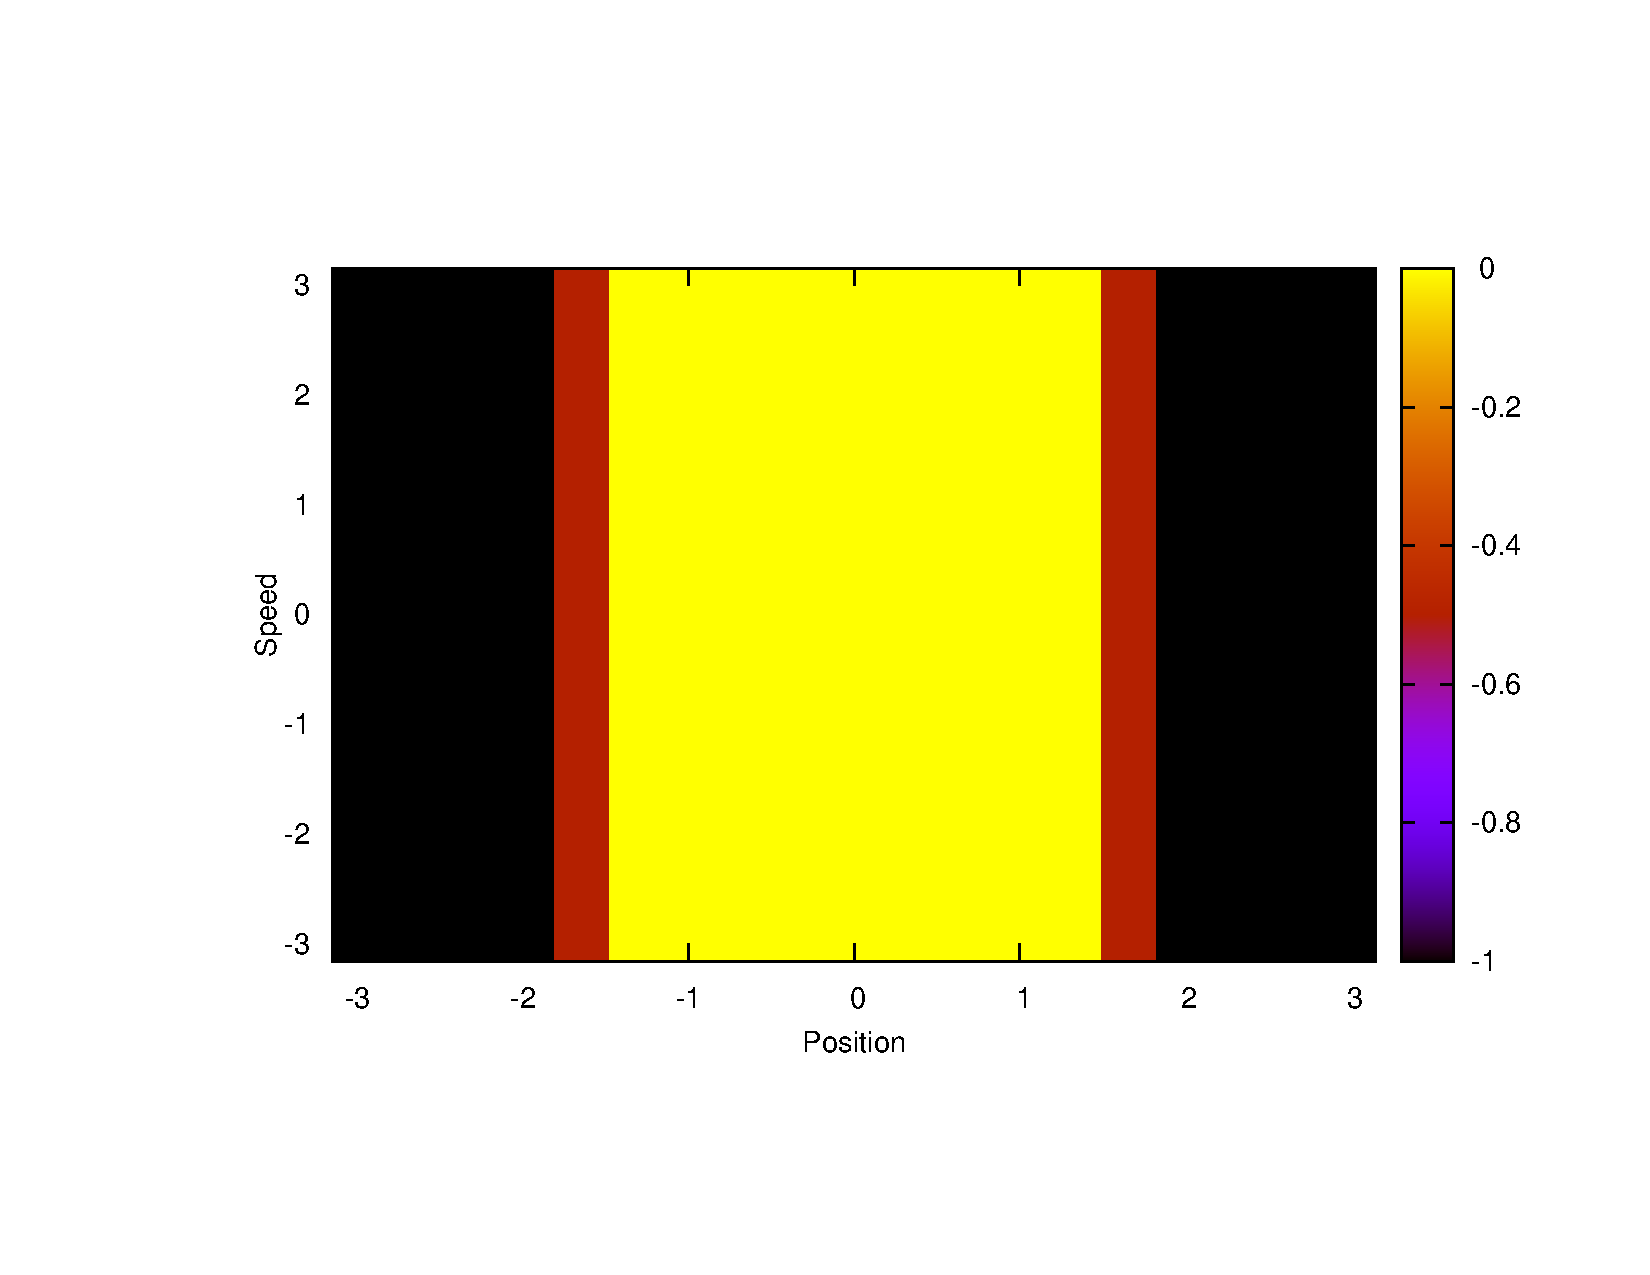
\includegraphics[width=1.2\textwidth]{LAFEM_Exp3_true_R.pdf}
       \caption{Récompense sur laquelle l'expert a été entraîné}
       \label{trueR.fig}
    \end{center}
\end{minipage}
\hfill
\begin{minipage}[t]{.4\linewidth}
    \begin{center}
       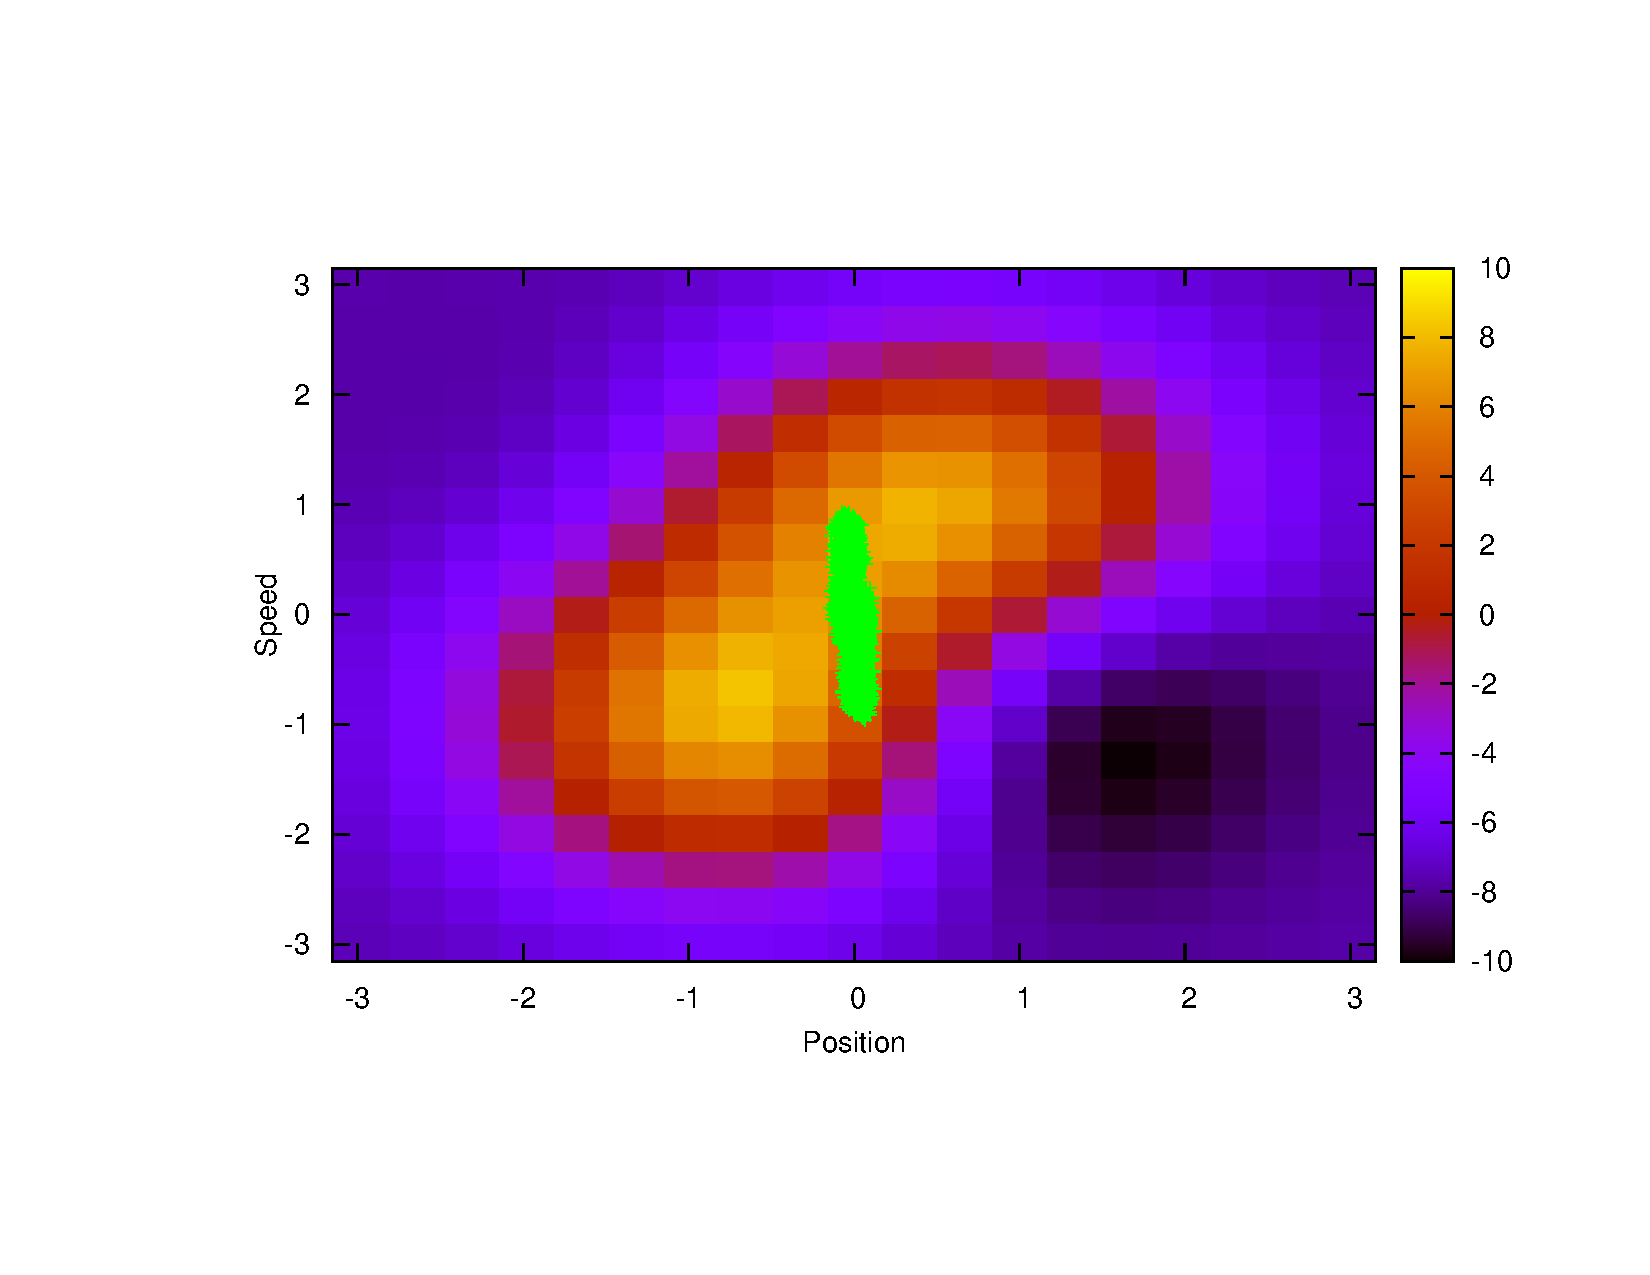
\includegraphics[width=1.2\textwidth]{LAFEM_Exp3_lafem_R.pdf}
       \caption{Récompense trouvée par LAFEM, en vert les positions occupées par l'expert.}
       \label{lafemR.fig}
    \end{center}
\end{minipage}\\
\begin{minipage}[t]{.4\linewidth}
    \begin{center}
       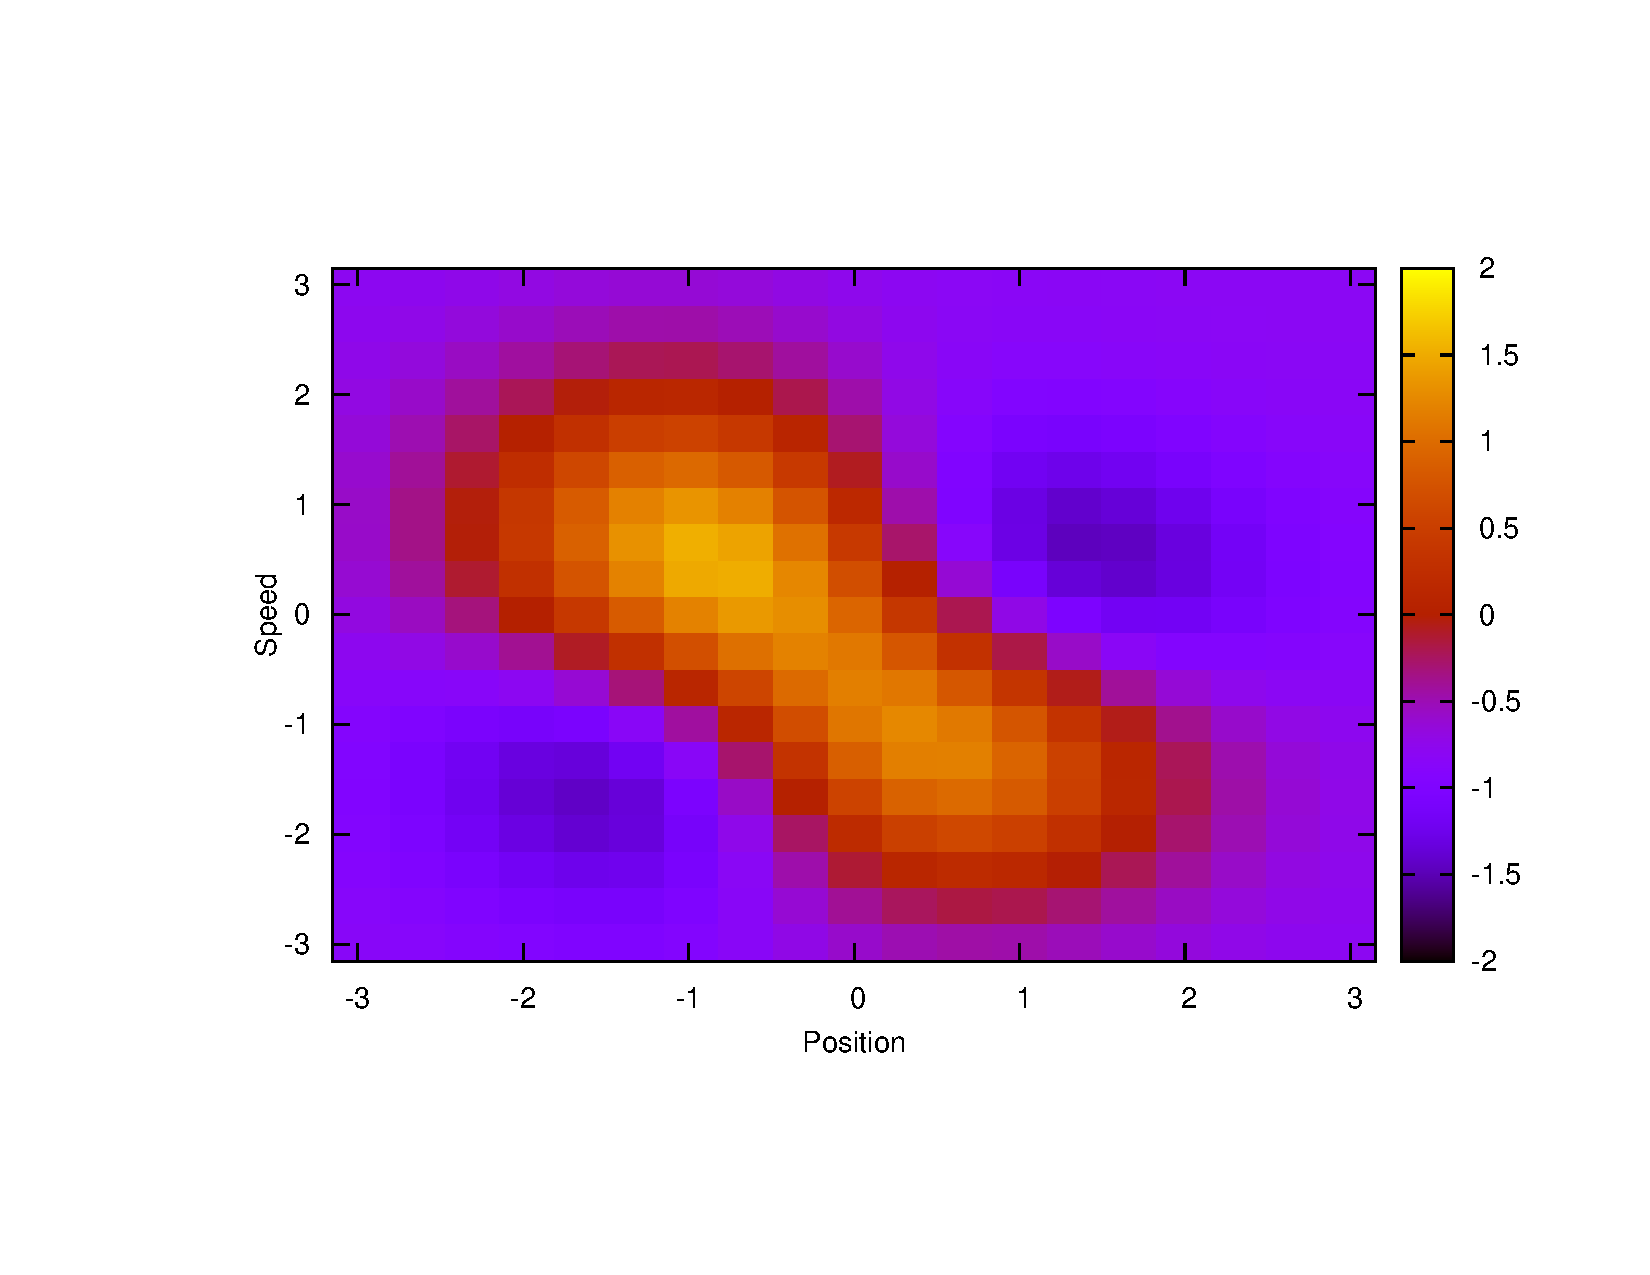
\includegraphics[width=1.2\textwidth]{LAFEM_Exp3_Vexpert.pdf}
       \caption{Fonction de valeur de l'expert}
       \label{trueV.fig}
    \end{center}
\end{minipage}
\hfill
\begin{minipage}[t]{.4\linewidth}
    \begin{center}
       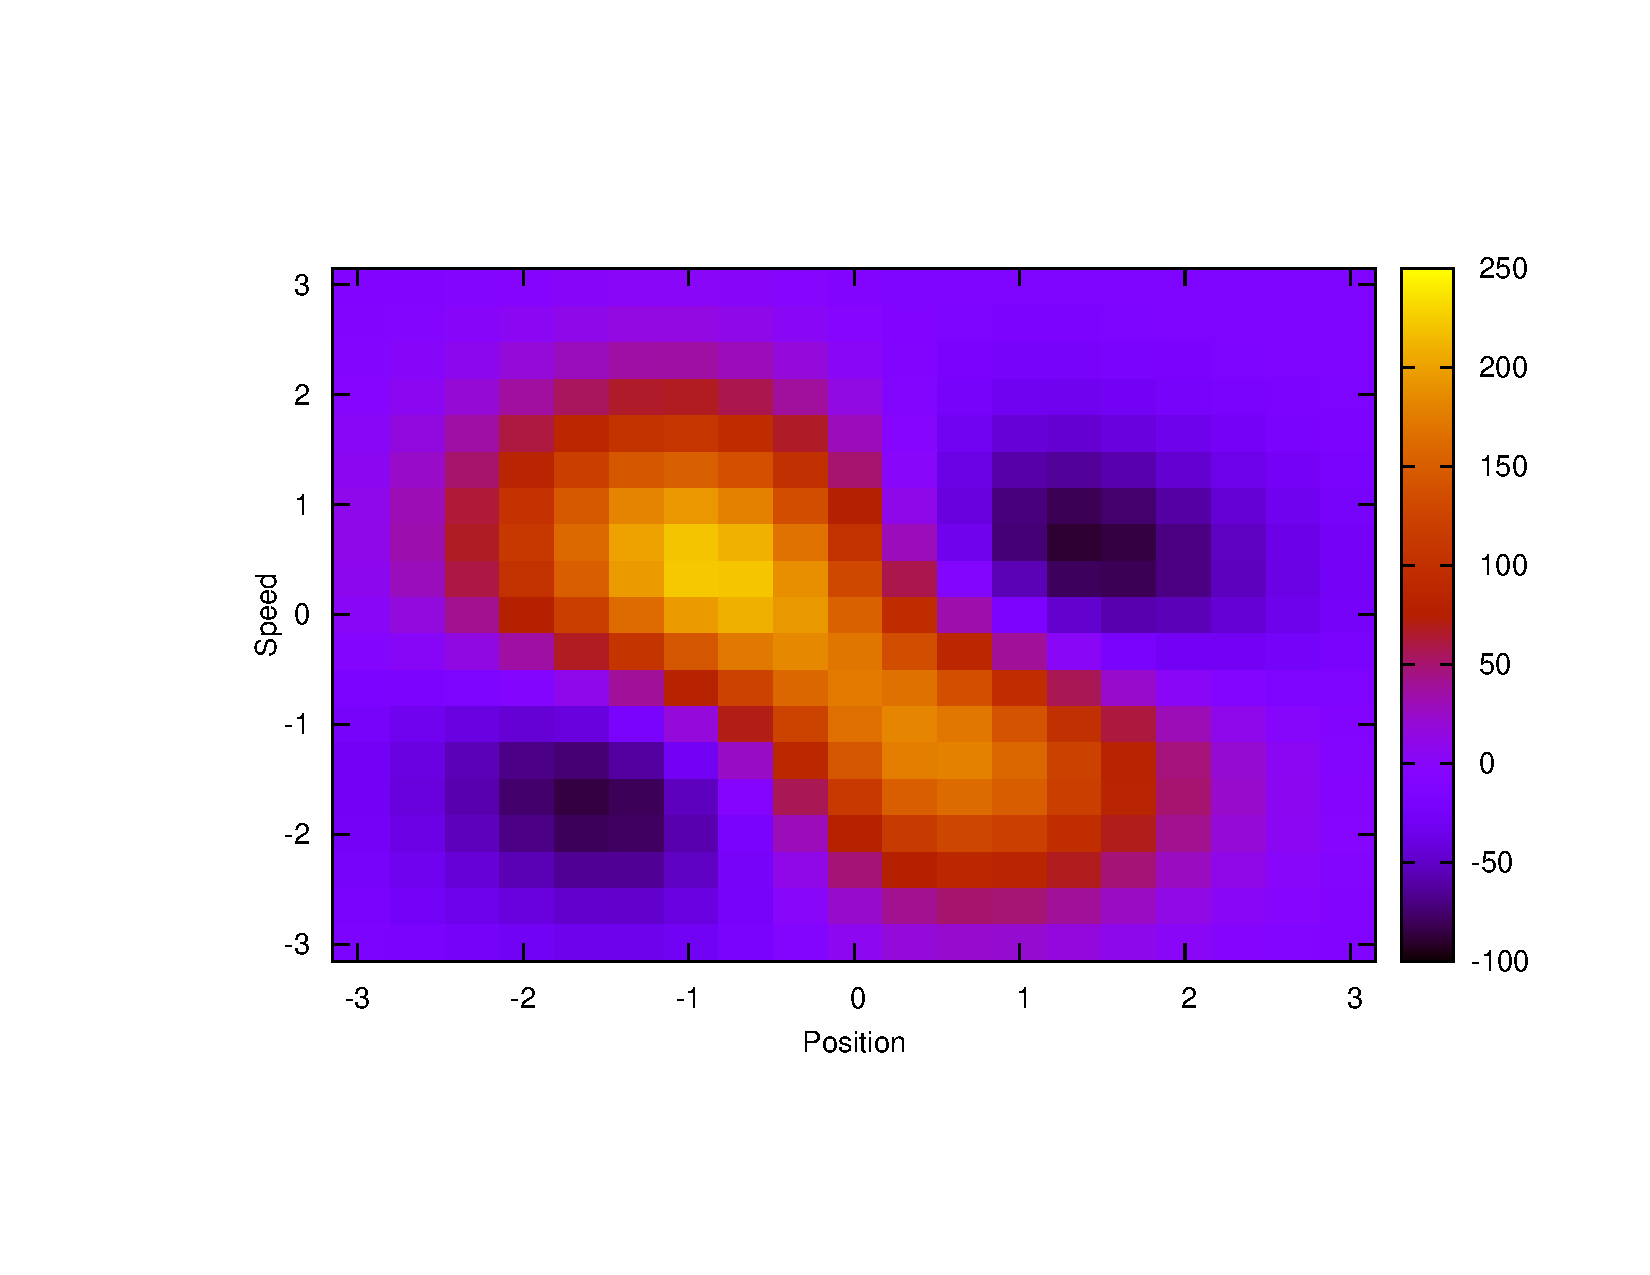
\includegraphics[width=1.2\textwidth]{LAFEM_Exp3_Vagent.pdf}
       \caption{Fonction de valeur de l'agent entraîné sur la récompense trouvée par LAFEM}
       \label{lafemV.fig}
    \end{center}
\end{minipage}\\
\end{figure}
Afin d'étudier le comportement de notre algorithmes, nous avons établi le protocole expérimental suivant :
\begin{itemize}
 \item créer une base de données $D_0$ de transitions aléatoires ;
 \item entraîner un expert en utilisant LSPI nourri avec ces transitions ( definissant ainsi $\pi_E : S\rightarrow A$) ;
 \item vérifier que l'expert est en mesure de balancer le pendule durant 3000 pas de temps ;
 \item créer une base de données $D_E$ de transitions de l'expert, contenant 10 trajectoires de 300 transitions chacune ;
 \item définir $l$ telle que $l(s,a) = 0$ si $a=\pi_E(s)$, $1$ sinon, $l$ est définie sur les états présents dans $D_E$ ;
 \item définir $\alpha(t) = 0.1,\forall t$ ;
 \item définir $D$ à partir des transitions $D_E$ en enlevant l'état d'arrivée ;
 \item initialiser $\omega_0 = [-1...-1]^T$ ;
 \item fixer $T=20$ ;
 \item définir $\mu_E(s,a) = E\left.\left[\sum\limits_{t=0}^\infty \gamma^t \phi(s)\right|s_0 = s, a_0 = a, \pi_E\right]$ comme étant en pratique $\hat\mu_E(s,a) =  \omega^T_{\pi_E}\phi(s,a), \omega_{\pi_E} = LSTD\mu(D_E)$ ;
 \item faire tourner LAFEM ;
 \item entrainer un agent sur le problème du pendule inversé, avec la récompense trouvée par LAFEM : définir $\pi : S\rightarrow A$ ;
 \item vérifier que l'agent parvient lui aussi à maintenir le pendule en équilibre durant 3000 pas de temps.
\end{itemize}

Si la fonction de récompense trouvée par LAFEM (figure \ref{lafemR.fig}) diffère de celle fournie à l'expert (figure \ref{trueR.fig}) on constate en revanche que les fonctions de valeurs sont très similaires (figures \ref{trueV.fig} et \ref{lafemV.fig}). Cela est une illustration du fait que le problème de l'IRL est mal posé en ceci qu'il n'y a pas qu'une seule récompense pouvant expliquer une politique.\\

Avec le nombre d'échantillons fournis par l'expert (3000 en 10 trajectoires de 300 transitions chacune), l'agent parvient systématiquement à maintenir le pendule en équilibre durant 5 minutes, ce qui est rappelons le notre critère de réussite.\\

Deux éléments méritent d'être notés. Tout d'abord la faible couverture de l'espace d'état offerte par les échantillons de l'expert. Ceux-ci sont portés en vert sur la Figure \ref{lafemR.fig} et l'on constate qu'ils n'occupent qu'une toute petite partie de l'espace : celle dans laquelle le pendule est proche de la verticale. En l'absence de données dans le reste de l'espace d'état il n'est pas possible de pouvoir y inférer avec certitude la récompense. Le second point à noter est que la "vraie" récompense ne se trouve pas dans l'espace d'hypothèse que notre algorithme explore, en effet les attributs proposés dans le problème du pendule inversé par \citet{lagoudakis2003least} consistent en un réseau de gaussiennes qui ne peuvent qu'approximer la fonction de récompense utilisée sans l'atteindre.\\

Malgré ces deux difficultés, notre algorithme parvient comme nous l'avons dit à extraire une récompense qui permet à un agent d'obtenir des performances similaires à celles de l'expert.\\

La différence dans les amplitudes des récompenses et des fonctions de valeurs n'est pas un problème, c'est en effet un résultat connu en apprentissage par renforcement que multiplier fonction de récompense ou fonction de valeur par une constante positive n'impacte pas les politiques.
\section{Conclusion and future work}
\begin{itemize}
\item On enlève les contraintes du domaine d'un seul coup,
\item Il ne reste que la sélection ou détection de features, mais ce n'est pas hors de portée
\item Faible complexité computationnelle
\item Faible complexité en échantillons
\item Il reste des tests à faire sur le Highway driving (Pour ICML ?) et sur des expériences dans la vraie vie (bras robot ?) pour comparer à l'existant
\end{itemize}
%
% Bibliographie
%
\bibliography{Biblio}

\end{document}

